%% Same trigger selection as summarized in~\Cref{tab:triggers_hadhad} is used and similar event selection is applied for the LQ \hadhad channel as for the HH \hadhad channel as described in~\Cref{subsec:selhh_hadhad}, and additional or modified selections are applied to select preferable higher momentum objects. The event selection for the LQ \hadhad channel is summarized in~\Cref{tab:lq_hadhad_event_selection} and the additional or modified selections are listed below.

Selections are applied to selects events compatible with containing a $bb\tau_{had}\tau_{had}$ final state.
All events passing the trigger selection must then meet the following requirements.

\begin{itemize}
\item At least two jets;
\item Exactly two $\tau$-leptons passing the `loose' identification criteria;
\item No electrons or muons in the event;
\item 1 or 2 $b$-tagged jets (using DL1r 77\% working point);
\item Opposite-sign charge between the two $\tau$-leptons;
\item At least one \bjet with \pT > \SI{45}{\GeV}. %\todo{Chris: maybe we
  % shoulddrop this selection?}
\item Applying $Z$ veto by excluding 40 GeV < $\mMMC_{\tau\tau}$ < 150 GeV.
\item The subleading \tauhad candidate is required to have $\pT > \SI{25}{\GeV}$
  (this is due to a $\SI{23}{\GeV}$ requirement in the HIGG4D3 derivation skim)
\item \MET is required to be greater than 100 GeV.
\end{itemize}

For STT events one of the two $\tau_{had}$ has to be matched to the object that fired the trigger, for DTT events both $\tau_{had}$ have to be matched to the objects that fired the trigger.

The \pt thresholds applied on the jets and the $\tau$-leptons depend on the trigger applied. The summary of the \pT thresholds applied is as follows:
\begin{itemize}
\item STT events: \tauhadvis are required to pass a trigger-dependent
  \pT threshold as described in
  \cref{sec:hadhad_trigger_selection}. Only if the event was not
  selected by the STT relevant for the particular run (even if the
  event was selected by a di-\tauhad trigger), it is checked whether
  the event passes the DTT selection (i.e.\ STT events are prioritized
  over DTT events).

\item DTT events in 2015-2016: The leading jet is required to have \pT >
  \SI{80}{\GeV} due to the additional jet requirement (J25) at L1 in 2016. This
  ensures that the L1 trigger is close to its efficiency plateau, minimizing the
  impact of a mismatch in trigger efficiency in data / MC.

\item DTT events in 2017-2018: Are categorised into two categories depending on
  the triggers to be checked: %\todo{Chris: need to check treatment of non-L1Topo trigger at the beginning of 2017}
  \begin{itemize}
  \item If leading and subleading jet $\pT > \SI{45}{\GeV}$: Event is considered a
    4J12 event. This cut ensures that the additional jet requirement at L1 (J12)
    is fulfilled.
  \item Else if leading jet $\pT > \SI{80}{\GeV}$ and $\dRtautau \leq 2.5$:
    Event is considered a L1Topo event. The jet \pT and \dRtautau cut ensure
    that the additional J25 and \dRtautau requirement at L1 are fulfilled.
  \end{itemize}
\end{itemize}

\begin{table}
  \centering
  \begin{tabular}{l|c} 
    \hline\hline
                                             & Criteria \\ \hline
    Trigger                                  & Single Tau Trigger or Di-Tau Trigger \\
    $N_{\ell}$                               & $=0$ \\
    $N_{\tauhad}$                            & $=2$ \\
    $N_{\mathrm{jets}}$                      & $\geq 2$ \\
    $N_{\mathrm{b-jets}}$                    & $=1$ or $=2$ (DL1r 77\% WP)\\
    $m_{MMC}$                                & $<40$ GeV or $>150$ GeV\\
    At least one b-jet $p_T$                 & $>45$ GeV \\
    $\tau_{\mathrm{had}}$ charges            & Opposite sign\\
    $E_{T}^{\mathrm{miss}}$                  & $> 100$ GeV \\
    \hline\hline
  \end{tabular}
  \caption{Event selection criteria for the LQ \hadhad channel.}
  \label{tab:lq_hadhad_event_selection}
\end{table}

%% \begin{itemize}
%%     \item The invariant mass requirement for the di-$\tau$ system of $\mMMC_{\tau\tau}$ > 60 $\GeV$ is not applied. Instead, applying $Z$ veto by excluding 40 GeV < $\mMMC_{\tau\tau}$ < 150 GeV.
%%     %% \item $s_T$ is required to be greater than 600 GeV.
%%     \item \MET is required to be greater than 100 GeV.
%%     \item One or two $b$-tagged jets are required.
%% \end{itemize} 

The $Z$ veto selection removes 95\% of $Z$+jets events while almost no loss of high mass LQ signal events. The \MET requirement reduces significant amount of multijet background. Events containing one or two $b$-tagged jets are inclusively treated as signal region. The event yields after applying the LQ \hadhad event selection is summarised in~\Cref{tab:LQHadHadYields} for backgrounds and in~\Cref{tab:LQHadHadYields_signal} for signal. The estimation of \ttbar with fake $\tau$s and multijet events is described in~\Cref{sec:bkgLQ}.

\begin{table}
\centering
\begin{tabular}{|c|c|c|c|c|}
\hline
\hline
SampleName & Entries & Integral & Error    & Error/Integ.\\
Fake       & 50029   & 42.5544  & 13.3786  & 0.314389\\
ttbarFF    & 116     & 16.7689  & 1.79812  & 0.107229\\
ttbarFT    & 2999    & 338.806  & 6.80948  & 0.0200985\\
ttbarTF    & 4307    & 618.382  & 10.1364  & 0.0163918\\
ttbar      & 15145   & 2321.82  & 19.8941  & 0.00856833\\
stopWtFF   & 10      & 1.27205  & 0.418383 & 0.328905\\
stopWtFT   & 232     & 29.7747  & 2.03509  & 0.0683495\\
stopWtTF   & 484     & 63.4372  & 3.04002  & 0.0479217\\
stopWt     & 1600    & 211.989  & 5.59653  & 0.0264\\
stoptFF    & 0       & 0        & 0        & 0\\
stoptFT    & 26      & 6.49854  & 1.36511  & 0.210064\\
stoptTF    & 24      & 5.21982  & 1.37138  & 0.262725\\
stopt      & 12      & 3.5321   & 1.14257  & 0.323481\\
stopsFF    & 0       & 0        & 0        & 0\\
stopsFT    & 6       & 0.225962 & 0.093998 & 0.415991\\
stopsTF    & 21      & 0.661816 & 0.14988  & 0.226468\\
stops      & 4       & 0.168106 & 0.0884309& 0.526041\\
Zbb        & 1       & 0.0152084& 0.0152084& 1\\
Zbc        & 0       & 0        & 0        & 0\\
Zbl        & 8       & 0.0409055& 0.0497236& 1.21557\\
Zcl        & 0       & 0        & 0        & 0\\
Zl         & 0       & 0        & 0        & 0\\
Zttbb      & 1236    & 25.8128  & 1.39126  & 0.053898\\
Zttbc      & 597     & 5.15543  & 0.610529 & 0.118424\\
Zttbl      & 4823    & 54.3552  & 1.99543  & 0.036711\\
Zttcc      & 372     & 2.72167  & 0.382479 & 0.140531\\
Zttcl      & 1148    & 5.954    & 0.588987 & 0.098923\\
Zttl       & 2261    & 2.153    & 0.743418 & 0.345294\\
Wtt        & 2109    & 61.3235  & 2.76479  & 0.0450854\\
WW         & 85      & 1.83874  & 0.424814 & 0.231035\\
WZ         & 313     & 3.84024  & 0.474338 & 0.123518\\
ZZ         & 145     & 1.16605  & 0.180758 & 0.155017\\
VH         & 2069    & 0.255066 & 0.00843544 & 0.0330717\\
bkg:       & 90182   & 3825.74  & & \\
data       & 3450    & 3450     & & \\
\hline
\hline
\end{tabular}
\caption{Pre-fit event yields for backgrounds in the LQ \hadhad signal region. Here, Zttjj represents the processes as $Z\rightarrow\tau\tau + jj$,
whereas Zjj represents  $Z\rightarrow ee/\mu\mu + jj$.}
\label{tab:LQHadHadYields}
\end{table}

\begin{table}
\centering
\begin{tabular}{|c|c|c|c|c|}
\hline
\hline
SampleName & Entries & Integral  &    Error    & Error/Integ.\\
LQ3Up300   &  3693   &   11611.8 &    373.784  & 0.0321901 \\
LQ3Up400   &  4476   &   3543.39 &    102.957  & 0.0290561 \\
LQ3Up500   & 17337   &   1405.91 &    18.8652  & 0.0134185 \\
LQ3Up600   &  6701   &   538.013 &    11.7529  &  0.021845 \\
LQ3Up700   &  7108   &   217.606 &    4.38101  & 0.0201327 \\
LQ3Up800   &  7417   &   98.8519 &    1.88928  & 0.0191122 \\
LQ3Up850   &  5249   &   62.7702 &    1.41402  & 0.0225269 \\
LQ3Up900   & 18170   &   44.2458 &   0.527333  & 0.0119183 \\
LQ3Up950   &  5464   &   30.2151 &   0.652541  & 0.0215965 \\
LQ3Up1000  &  5351   &   20.4643 &   0.453636  & 0.0221671 \\
LQ3Up1050  &  5476   &    14.105 &   0.312004  & 0.0221202 \\
LQ3Up1100  &  5334   &   9.82703 &    0.21345  & 0.0217207 \\
LQ3Up1150  &  5162   &    6.6657 &   0.145919  &  0.021891 \\
LQ3Up1200  &  5265   &    4.8194 &   0.104777  & 0.0217407 \\
LQ3Up1250  &  2521   &   3.64774 &   0.112072  & 0.0307236 \\
LQ3Up1300  & 13799   &   2.57844 &   0.033844  & 0.0131258 \\
LQ3Up1350  &  1232   &   1.82472 &  0.0836093  & 0.0458204 \\
LQ3Up1400  &  1193   &   1.35815 &  0.0598979  & 0.0441025 \\
LQ3Up1450  &  1171   &  0.992608 &  0.0433566  & 0.0436795 \\
LQ3Up1500  &  1201   &  0.691491 &  0.0316072  & 0.0457088 \\
LQ3Up1550  &   762   &  0.610432 &  0.0327674  &  0.053679 \\
LQ3Up1600  &   651   &  0.366938 &  0.0216716  & 0.0590607 \\
LQ3Up1700  &  5079   &  0.211028 & 0.00445163  &  0.021095 \\
LQ3Up1800  &   616   &  0.103486 & 0.00642085  & 0.0620455 \\
LQ3Up1900  &   628   & 0.0642773 & 0.00371324  &  0.057769 \\
LQ3Up2000  &   649   & 0.0346446 & 0.00217091  & 0.0626623 \\
\hline
\hline
\end{tabular}
\caption{Pre-fit event yields for signals in the LQ \hadhad signal region. Here, Zttjj represents the processes as $Z\rightarrow\tau\tau + jj$,
whereas Zjj represents  $Z\rightarrow ee/\mu\mu + jj$.}
\label{tab:LQHadHadYields_signal}
\end{table}

\Cref{fig:selection_lq_hadhad:kinematic_variables} shows some kinematic variables in the signal region.
%Although individual kinematic variables do not have enough power to discriminate the signal and background events, a conservative blinding strategy is taken.
For \pT, \MET and $s_T$, quadratic sum of $S/\sqrt{B}$ is calculated from left to right, and when it exceeds 0.5, data is blinded from that bin.
Here signal sample of $m_{LQ} = 1100 GeV$ is considered.

\begin{figure}[!h]
  \centering
  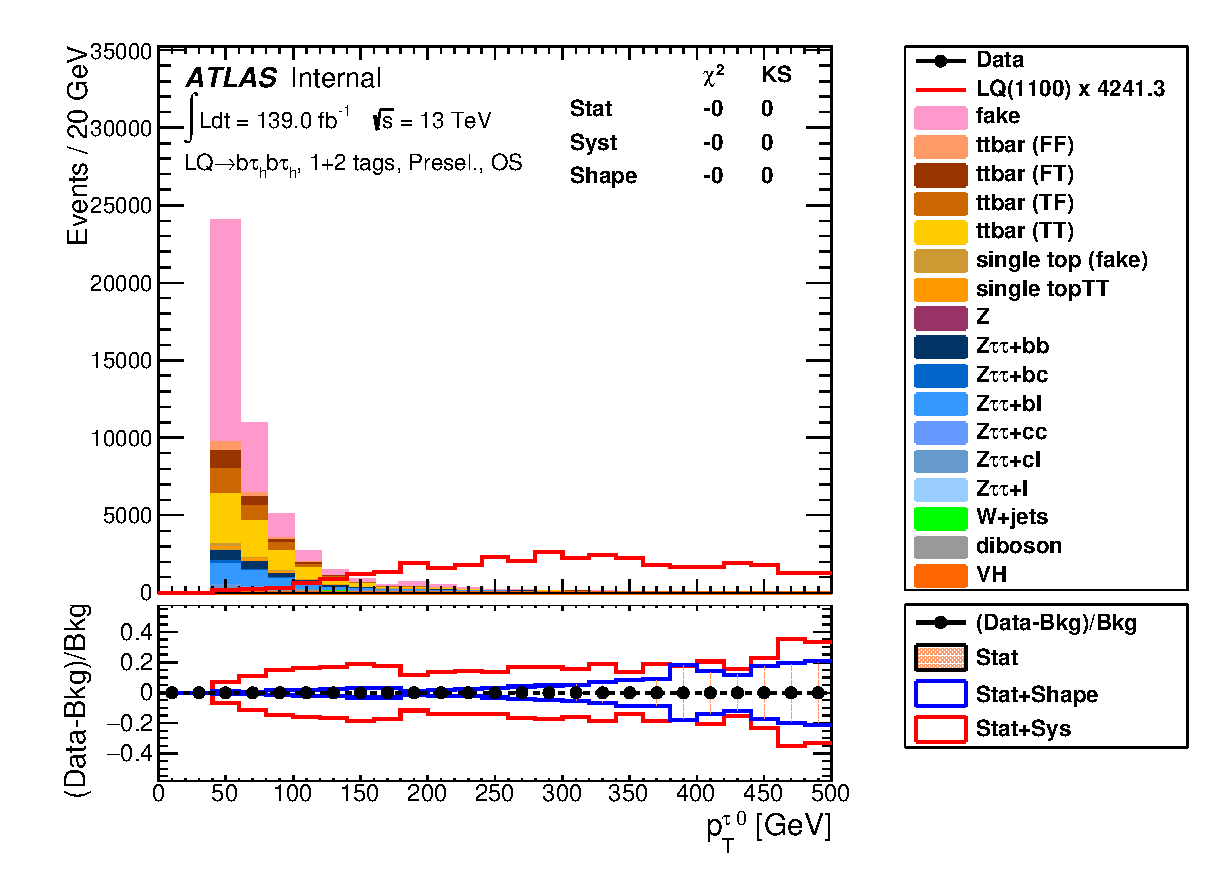
\includegraphics[width=0.4\textwidth]{figures/selection/lq3/hadhad/Plots_SR/C_3tag2pjet_0ptv_OS_Tau0Pt.eps} 
  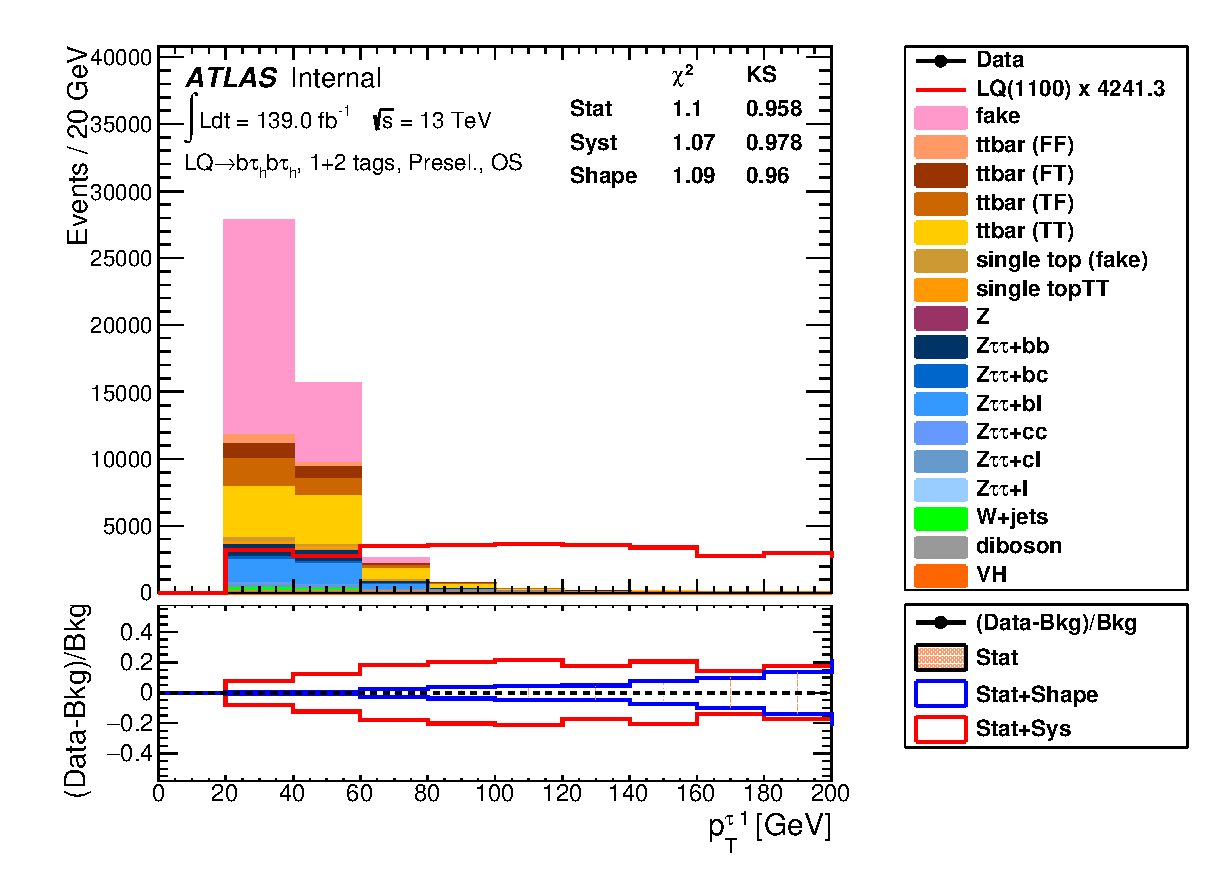
\includegraphics[width=0.4\textwidth]{figures/selection/lq3/hadhad/Plots_SR/C_3tag2pjet_0ptv_OS_Tau1Pt.eps} \\
  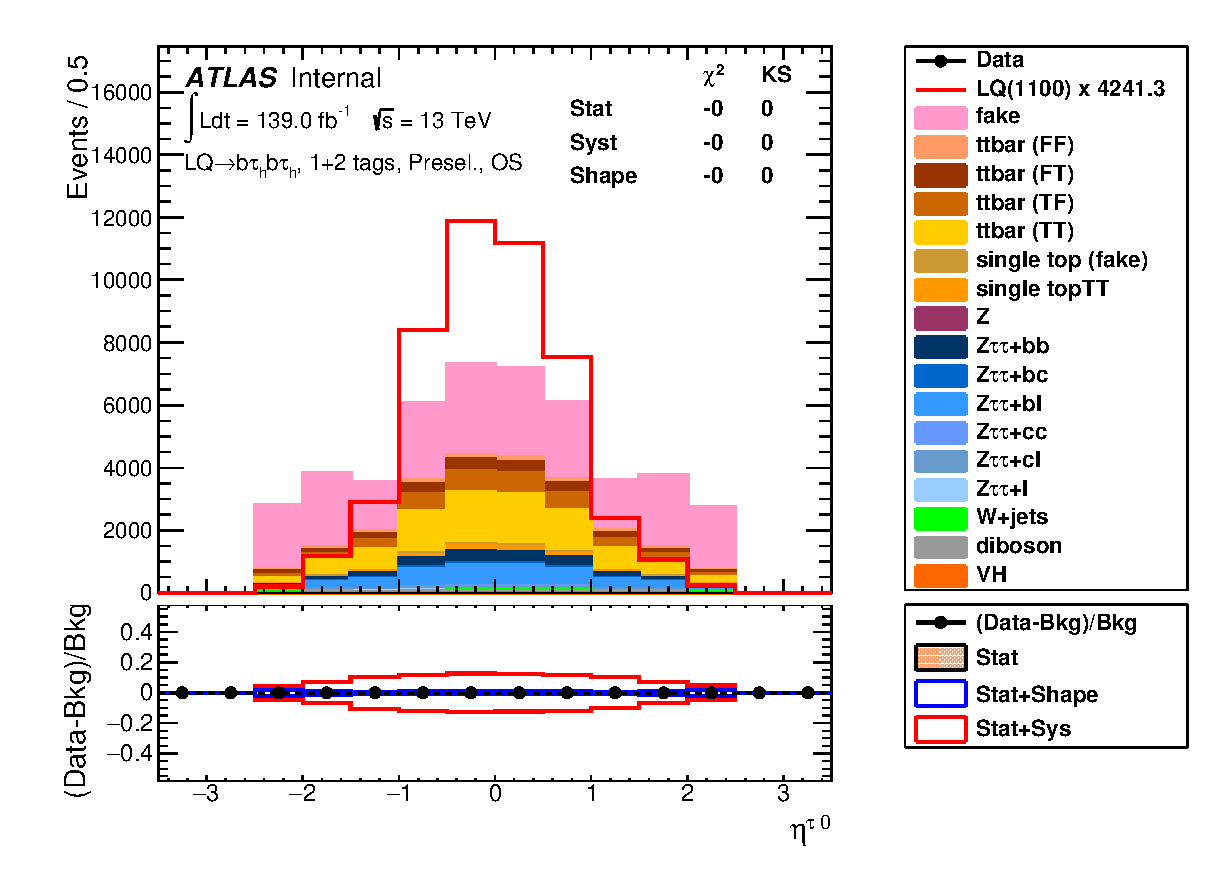
\includegraphics[width=0.4\textwidth]{figures/selection/lq3/hadhad/Plots_SR/C_3tag2pjet_0ptv_OS_Tau0Eta.eps} 
  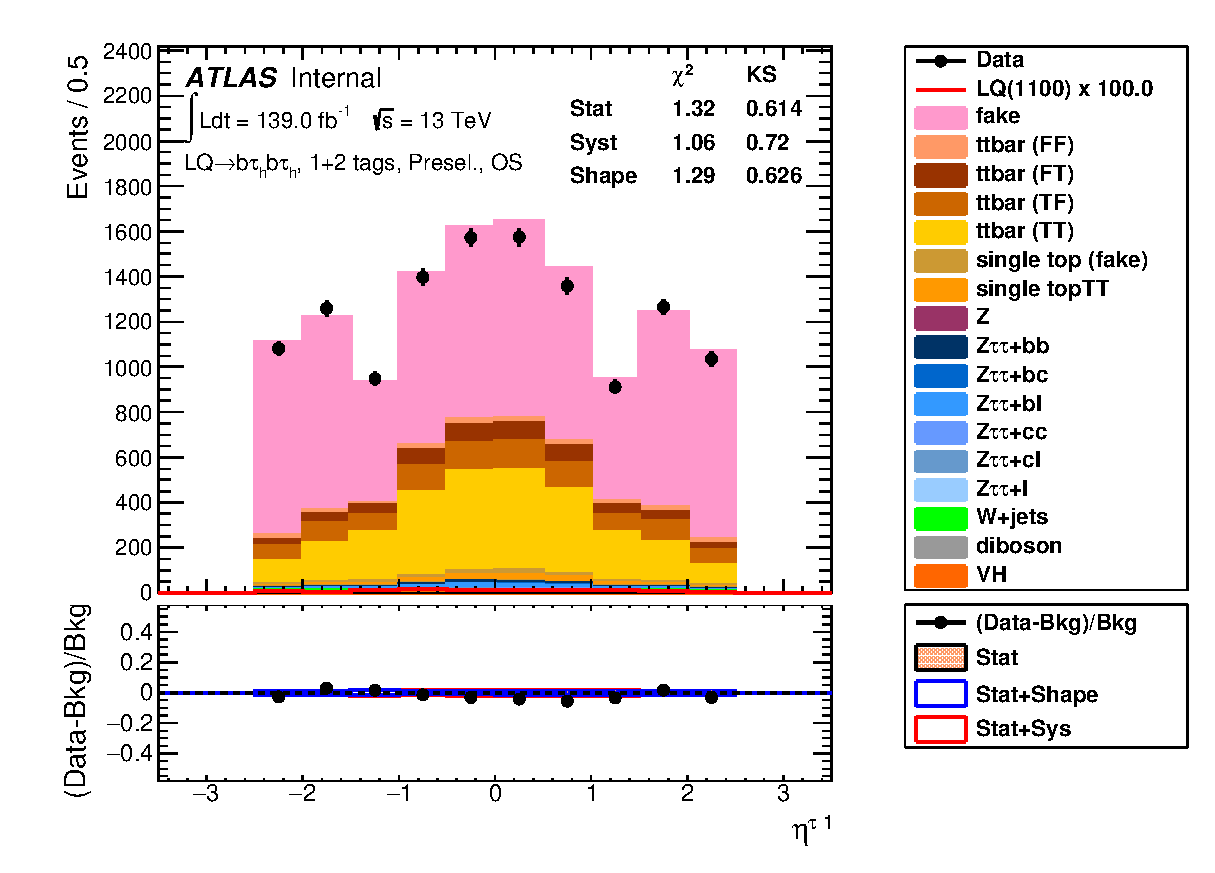
\includegraphics[width=0.4\textwidth]{figures/selection/lq3/hadhad/Plots_SR/C_3tag2pjet_0ptv_OS_Tau1Eta.eps} \\
  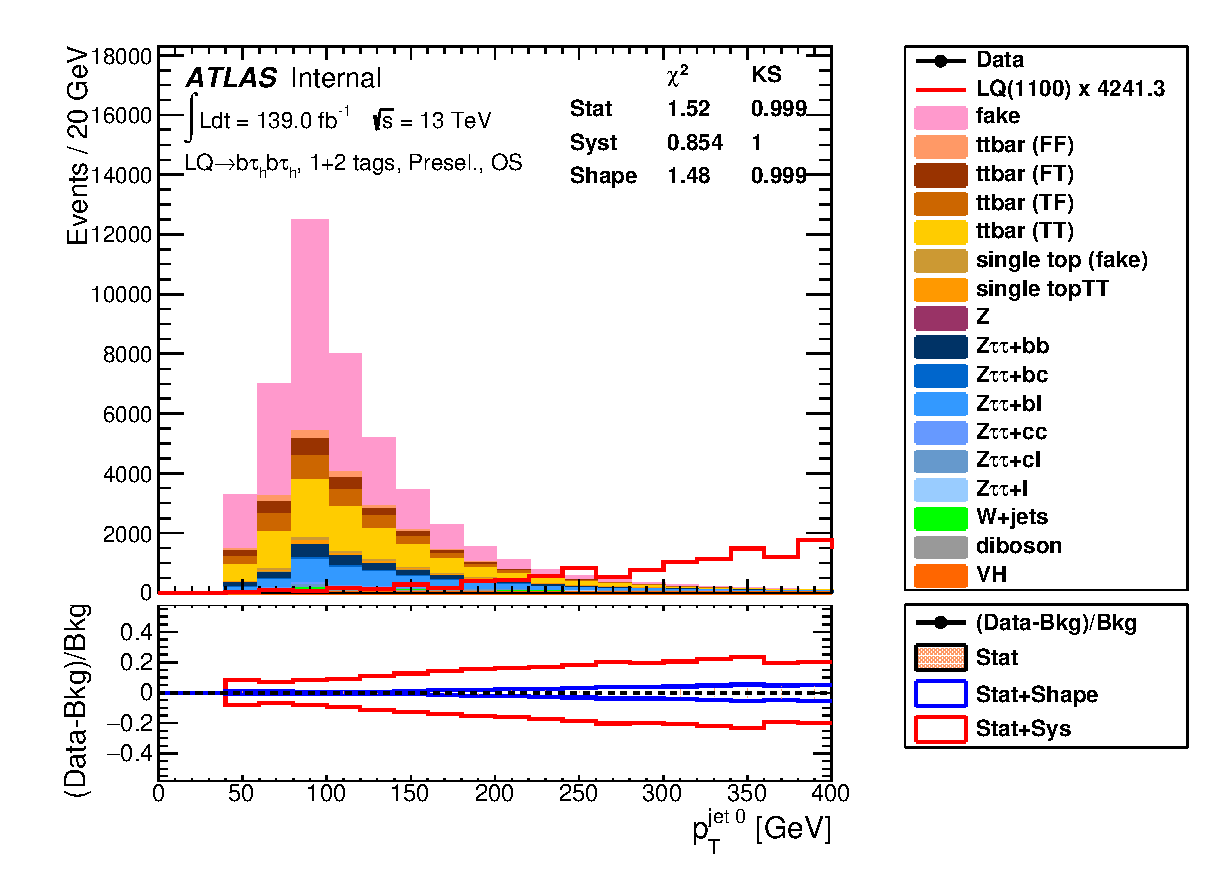
\includegraphics[width=0.4\textwidth]{figures/selection/lq3/hadhad/Plots_SR/C_3tag2pjet_0ptv_OS_Jet0Pt.eps} 
  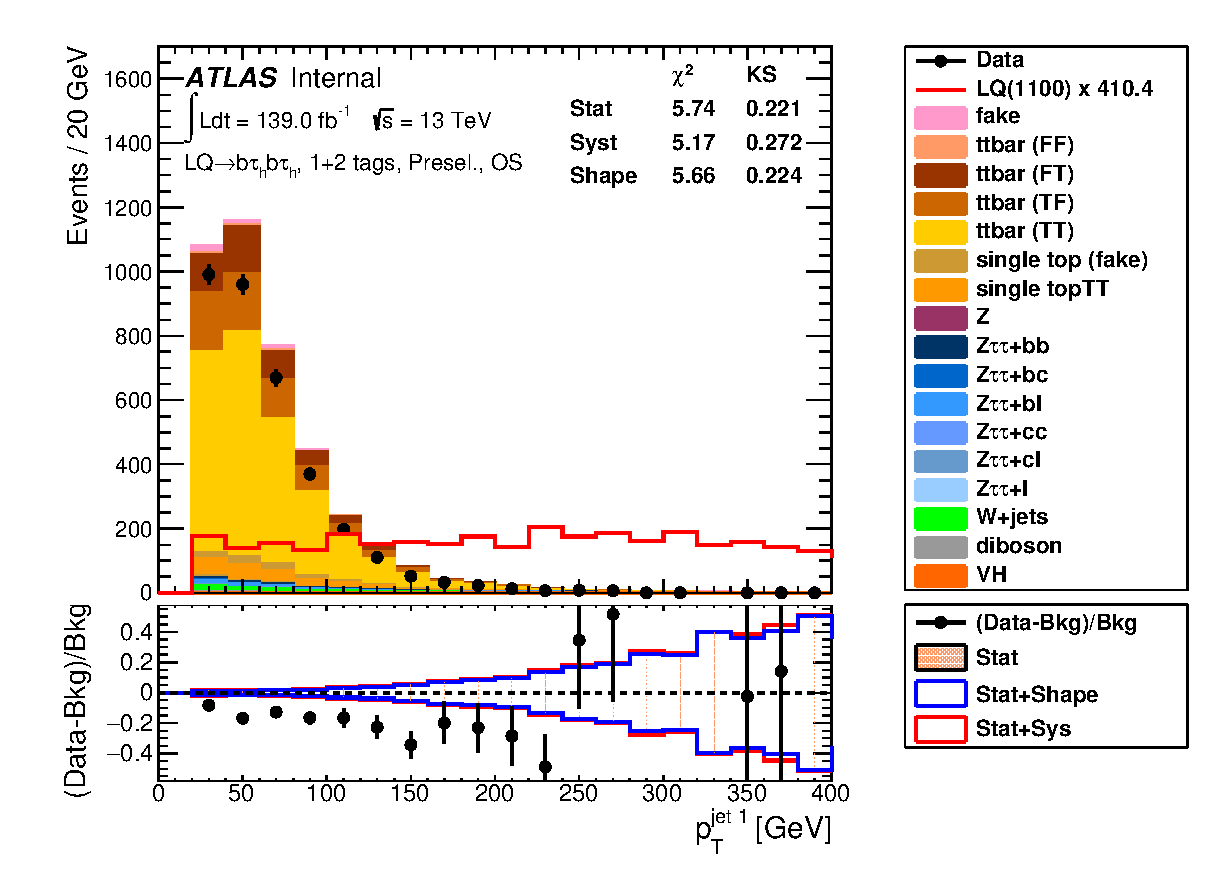
\includegraphics[width=0.4\textwidth]{figures/selection/lq3/hadhad/Plots_SR/C_3tag2pjet_0ptv_OS_Jet1Pt.eps} \\
  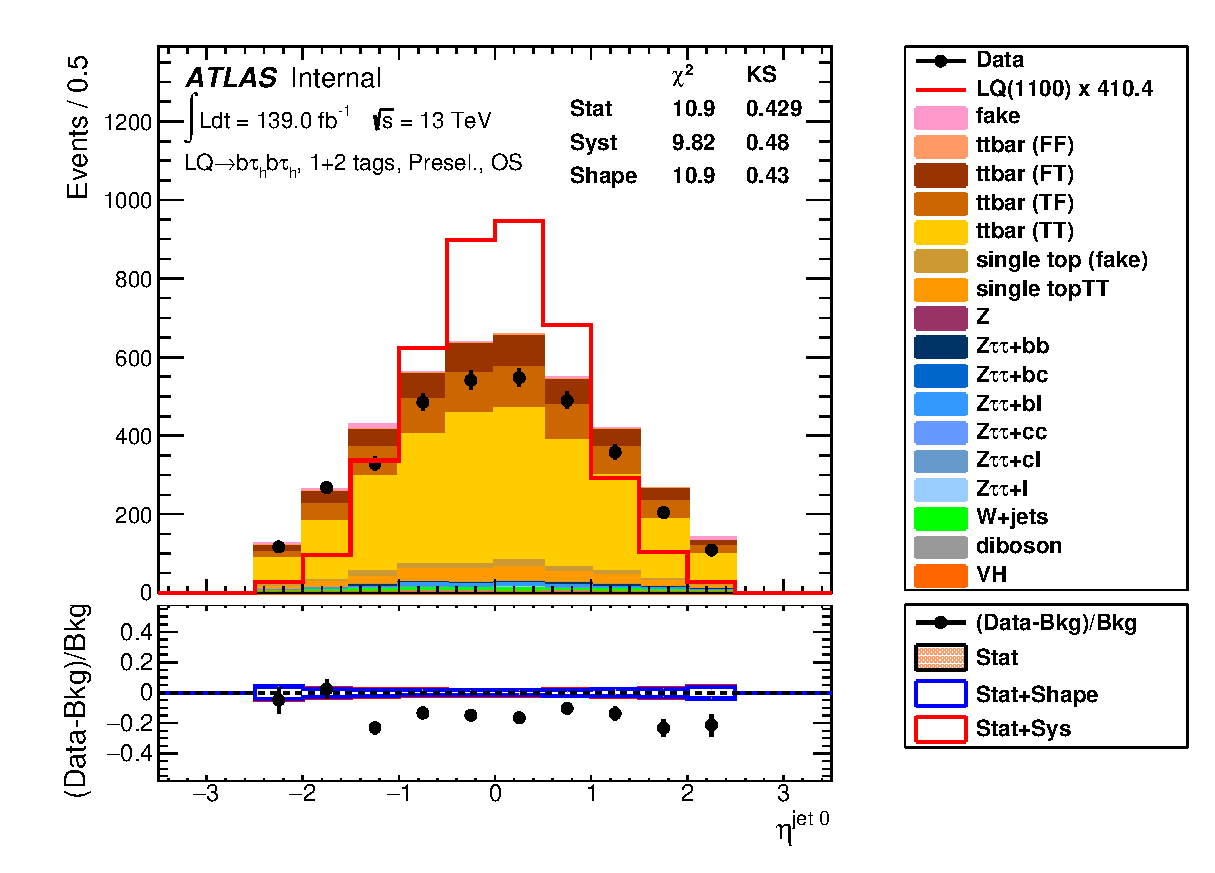
\includegraphics[width=0.4\textwidth]{figures/selection/lq3/hadhad/Plots_SR/C_3tag2pjet_0ptv_OS_Jet0Eta.eps} 
  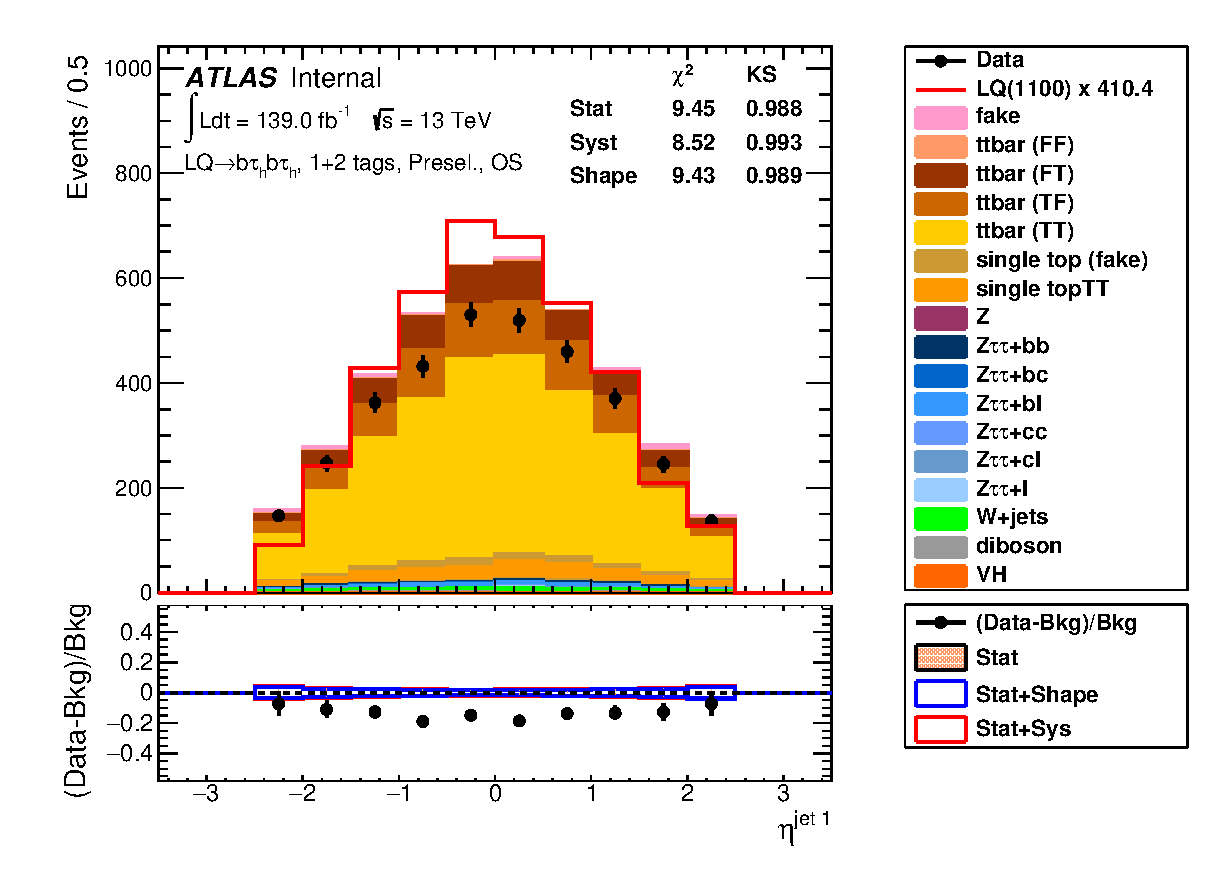
\includegraphics[width=0.4\textwidth]{figures/selection/lq3/hadhad/Plots_SR/C_3tag2pjet_0ptv_OS_Jet1Eta.eps} \\
  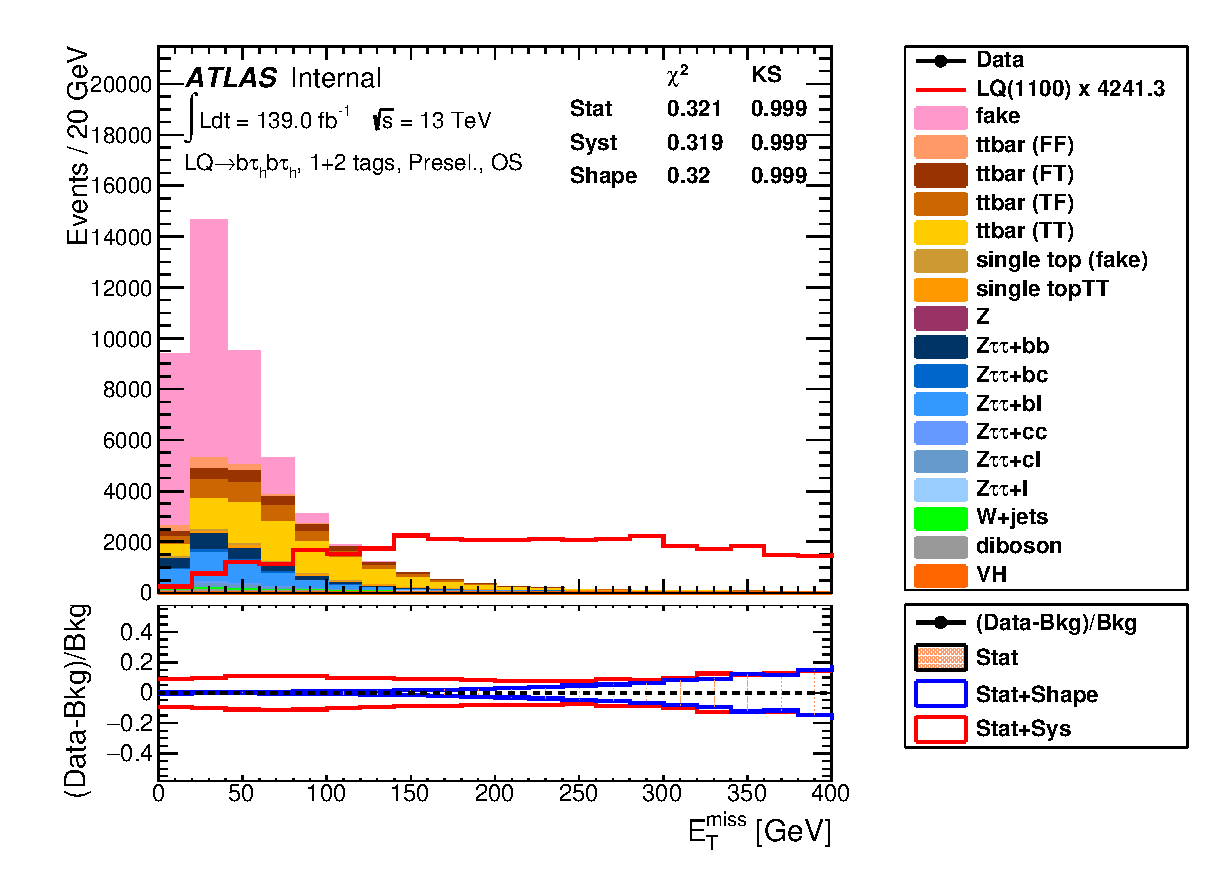
\includegraphics[width=0.4\textwidth]{figures/selection/lq3/hadhad/Plots_SR/C_3tag2pjet_0ptv_OS_MET.eps} 
  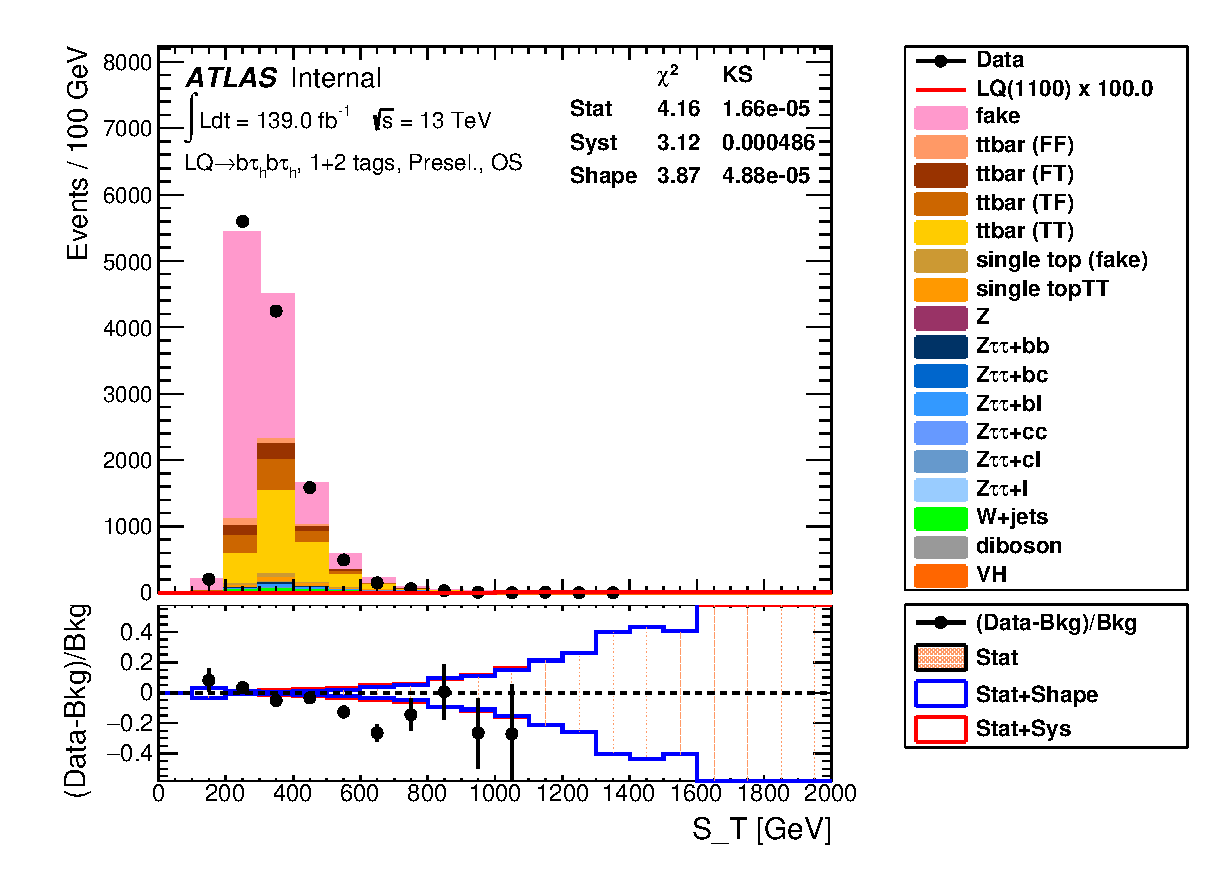
\includegraphics[width=0.4\textwidth]{figures/selection/lq3/hadhad/Plots_SR/C_3tag2pjet_0ptv_OS_SR_sT.eps} 
  \caption{Kinematic variable distributions in the signal region. The grey colored band show the blinded region. Here, bins where the quadratic sum of $S/\sqrt{B}$ is greater than 0.2 are blinded for the 1100 GeV signal. $S$ is the number of signal yields , and $\sqrt{B}$ is the square of the number of backgrounds in the bin respectively.}
  \label{fig:selection_lq_hadhad:kinematic_variables}
\end{figure}


The event selection in the signal regions in the LQ analysis, i.e. the $p_T$ requirements and the object multiplicities, are summarised in Table~\ref{tab:LQEventSelection}.

\begin{table}[!h]
\centering
\begin{tabular}{c|c|c}
 \toprule
  \lephad\ channel & \multicolumn{2}{c}{\hadhad\ channel}  \\[0.2em]
 \toprule
  \multicolumn{3}{c}{Trigger selection:} \\[0.5em]
 Single-$\ell$ trigger            & Single-\tauhad\ trigger  & Di-\tauhad\ trigger  \\
 SLT                              & STT                      & DTT                  \\\cmidrule[0.2pt]{1-3}

 % light-lepton selection
 \multicolumn{3}{c}{$e/\mu$ selection:} \\ [0.5em]
 \small One tight $e$ or medium $\mu$ & \multicolumn{2}{c}{\small No loose $e/\mu$ with $p_T>7$~GeV}  \\[0.2em]
 \small $p_T^{e}>25,27$ GeV    &  &  \\
 \small $p_T^{\mu}>22,27$ GeV  &  &  \\\cmidrule[0.2pt]{1-3}

 % tau_had selection
 \multicolumn{3}{c}{\tauhad\ selection:} \\ [0.5em]
 \small One loose \tauhad\ ($|\eta|<2.3$) & \multicolumn{2}{c}{\small Two loose \tauhad\ ($|\eta|<2.5$)}  \\[0.2em]
 \small $p_T^{\tau}>100$ GeV              & \small $p_T>100,140,180\text{ }(25)$~GeV & \small $p_T>40\text{ }(30)$ GeV \\\cmidrule[0.2pt]{1-3}


 % jet selection
 \multicolumn{3}{c}{Jet selection {\small($\geq2$ central jets)}:} \\[0.5em]

 \small $p_T>60\text{ }(20)$ GeV & \small $p_T>45\text{ }(20)$ GeV & \small \textbf{2015 $+$ 2016:}  \\
                                 &                                 & \small $p_T>80\text{ }(20)$ GeV \\[0.5em]

                                 &                                 & \small \textbf{2017 $+$ 2018:}  \\
                                 &                                 & \small\textit{``L14j12'' seed:} \\
                                 &                                 & \small $p_T>45\text{ }(45)$ GeV \\[0.5em]
                                 &                                 & \small\textit{``L1Topo'' seed:} \\
                                 &                                 & \small $p_T>80\text{ }(20)$ GeV \\
                                 &                                 & \small and $\Delta R_{\tau\tau}<2.5$\\[0.5em]\cmidrule[0.2pt]{1-3}

% \midrule
 \multicolumn{3}{c}{Additional selection:}                                                 \\[0.5em]
 \multicolumn{3}{c}{\small Opposite-sign electric charges of $e/\mu/$\tauhad\ and \tauhad} \\
 \multicolumn{3}{c}{\small 1 or 2 $b$-tagged jets (77\% efficiency)}                       \\
 \multicolumn{3}{c}{\small $E_{T}^{\mathrm{miss}} > 100$~GeV} \\
                                 & \multicolumn{2}{c}{\small 40~GeV $ < m_{\tau\tau}^{\mathrm{MMC}} < 150 $~GeV} \\
 \small $s_T$ > 600~GeV          &                                 &                       \\ 
 \bottomrule
\end{tabular}
\caption{Summary of the signal region event selection in the LQ analysis, shown separately for the three trigger categories. In cases when several objects of the same type are required, the respective $p_T$ threshold for the leading (sub-leading) object is given outside (within) parentheses. For the SLT category, the $p_T$ requirements depend on the data-taking period, therefore several thresholds are listed, separated by commas. In the DTT trigger category, several different L1 seeds are used for the 2017 and 2018 data-taking periods, impacting the jet selection criteria, and thus the jet $p_T$ thresholds are summarised separately for the each L1 seed.
}
\label{tab:LQEventSelection}
\end{table}

\FloatBarrier


%% \begin{figure}[!h]
%%   \centering
%%   \includegraphics[width=0.4\textwidth]{figures/selection/lq3/Merged_TauHH_LQ_1618_No4_Final_20201026_Preselection_incl12tag_Tau0Pt.pdf} 
%%   \includegraphics[width=0.4\textwidth]{figures/selection/lq3/Merged_TauHH_LQ_1618_No4_Final_20201026_Preselection_incl12tag_Tau1Pt.pdf} \\
%%   \includegraphics[width=0.4\textwidth]{figures/selection/lq3/Merged_TauHH_LQ_1618_No4_Final_20201026_Preselection_incl12tag_Jet0Pt.pdf} 
%%   \includegraphics[width=0.4\textwidth]{figures/selection/lq3/Merged_TauHH_LQ_1618_No4_Final_20201026_Preselection_incl12tag_Jet1Pt.pdf} \\
%%   \includegraphics[width=0.4\textwidth]{figures/selection/lq3/Merged_TauHH_LQ_1618_No4_Final_20201026_Preselection_incl12tag_sT.pdf}
%%   \caption{Kinematic variable distributions in the signal region. The grey colored band show the blinded region. Here, bins where the $S/\sqrt{B}$ is greater than 0.1 are blinded for the 1000 GeV signal. $S$ is the number of signal yields , and $\sqrt{B}$ is the square of the number of backgrounds in the bin respectively.}
%%   \label{fig:selection_lq_hadhad:kinematic_variables}
%% \end{figure}

\clearpage 


%There are two differences between the \hadhad channels of di-Higgs and LQLQ. One is that the requirement for invariant mass of the di-$\tau$ system is not applied in the LQLQ channel since correct pairing for a LQ is from $b\tau$, and the other is that events with 1 or 2 b-jets are considered as signal region for the LQLQ channel while only events with 2 b-jets are for the di-Higgs channel.

% The invariant mass requirement for the di-$\tau$ system is not applied in this channel since correct pairing for a LQ is from $b\tau$
